\documentclass[a4paper]{article}
\usepackage{amsmath, amsfonts}
\usepackage{tikz}
\usetikzlibrary{arrows, shapes}
\usetikzlibrary{decorations.pathmorphing}
\usetikzlibrary{calc,arrows.meta,positioning}

\begin{document}

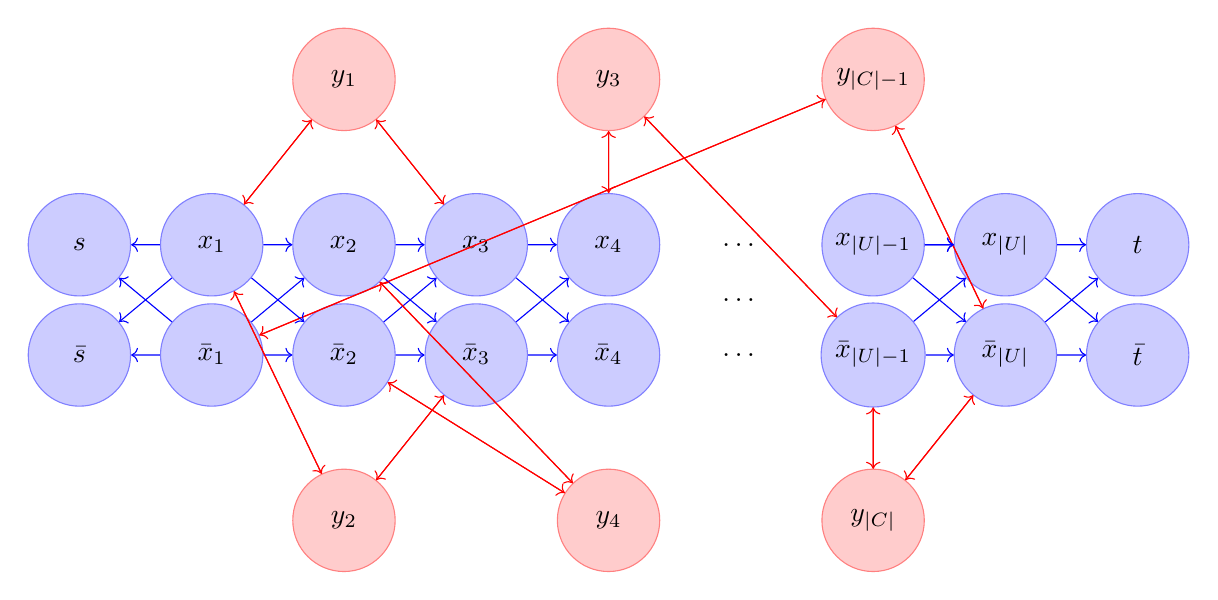
\begin{tikzpicture}[scale=1.4]
	\begin{scope}[circle,minimum size=13mm]
		\draw
		(0, 0.5) node[draw=blue!50, fill=blue!20] (s){$s$}
		(0, -0.5) node[draw=blue!50, fill=blue!20] (-s){$\bar{s}$}
		(1.2, -0.5) node[draw=blue!50, fill=blue!20] (-1){$\bar{x}_{1}$}
		(1.2, 0.5) node[draw=blue!50, fill=blue!20] (1){$x_{1}$}
		(2.4, -0.5) node[draw=blue!50, fill=blue!20] (-2){$\bar{x}_{2}$}
		(2.4, 0.5) node[draw=blue!50, fill=blue!20] (2){$x_{2}$}
		(3.6, -0.5) node[draw=blue!50, fill=blue!20] (-3){$\bar{x}_{3}$}
		(3.6, 0.5) node[draw=blue!50, fill=blue!20] (3){$x_{3}$}
		(4.8, -0.5) node[draw=blue!50, fill=blue!20] (-4){$\bar{x}_{4}$}
		(4.8, 0.5) node[draw=blue!50, fill=blue!20] (4){$x_{4}$}
		(7.2, -0.5) node[draw=blue!50, fill=blue!20] (-6){$\bar{x}_{|U|-1}$}
		(7.2, 0.5) node[draw=blue!50, fill=blue!20] (6){$x_{|U|-1}$}
		(8.4, -0.5) node[draw=blue!50, fill=blue!20] (-7){$\bar{x}_{|U|}$}
		(8.4, 0.5) node[draw=blue!50, fill=blue!20] (7){$x_{|U|}$}
		(9.6, 0.5) node[draw=blue!50, fill=blue!20] (t){$t$}
		(9.6, -0.5) node[draw=blue!50, fill=blue!20] (-t){$\bar{t}$}
		(2.4, 2) node[draw=red!50, fill=red!20] (1000){$y_{1}$}
		(2.4, -2) node[draw=red!50, fill=red!20] (1001){$y_{2}$}
		(4.8, 2) node[draw=red!50, fill=red!20] (1002){$y_{3}$}
		(4.8, -2) node[draw=red!50, fill=red!20] (1003){$y_{4}$}
		(7.2, 2) node[draw=red!50, fill=red!20] (1004){$y_{|C|-1}$}
		(7.2, -2) node[draw=red!50, fill=red!20] (1005){$y_{|C|}$};
	\end{scope}

	\node at ($(4)!.5!(6)$) {\ldots};
	\node at ($(-4)!.5!(-6)$) {\ldots};
	\node at ($(4)!.5!(-6)$) {\ldots};

	\begin{scope}[->]
		\draw[blue] (-1) to (2);
		\draw[blue] (-1) to (-2);
		\draw[red] (-1) to (1004);
		\draw[red] (1004) to (-1);
		\draw[blue] (1) to (-2);
		\draw[blue] (-2) to (3);
		\draw[blue] (-2) to (-3);
		\draw[red] (-2) to (1003);
		\draw[red] (1003) to (-2);
		\draw[blue] (2) to (-3);
		\draw[blue] (-3) to (4);
		\draw[red] (-3) to (1001);
		\draw[red] (1001) to (-3);
		\draw[blue] (-3) to (-4);
		\draw[blue] (3) to (-4);
		\draw[blue] (-6) to (7);
		\draw[blue] (-6) to (-7);
		\draw[red] (-6) to (1002);
		\draw[red] (-6) to (1005);
		\draw[red] (1002) to (-6);
		\draw[red] (1005) to (-6);
		\draw[blue] (6) to (-7);
		\draw[red] (-7) to (1004);
		\draw[red] (-7) to (1005);
		\draw[red] (1004) to (-7);
		\draw[red] (1005) to (-7);
		\draw[blue] (1) to (2);
		\draw[red] (1) to (1000);
		\draw[red] (1) to (1001);
		\draw[red] (1000) to (1);
		\draw[red] (1001) to (1);
		\draw[blue] (2) to (3);
		\draw[red] (2) to (1003);
		\draw[red] (1003) to (2);
		\draw[blue] (3) to (4);
		\draw[red] (3) to (1000);
		\draw[red] (1000) to (3);
		\draw[red] (4) to (1002);
		\draw[red] (1002) to (4);
		\draw[blue] (6) to (7);
		\draw[blue] (6) to (7);
		\draw[blue] (7) to (t);
		\draw[blue] (-7) to (t);
		\draw[blue] (7) to (-t);
		\draw[blue] (-7) to (-t);
		\draw[blue] (1) to (s);
		\draw[blue] (-1) to (s);
		\draw[blue] (1) to (-s);
		\draw[blue] (-1) to (-s);
	\end{scope}
\end{tikzpicture}

\end{document}